\documentclass[a4paper, 11pt]{article}
\usepackage{comment} % enables the use of multi-line comments (\ifx \fi) 
\usepackage{fullpage} % changes the margin
\usepackage{vhistory}
\usepackage{enumitem}
\usepackage{listings}
\usepackage{color}
\usepackage{enumitem}
\usepackage{pdfpages}

\newlength{\drop}
\newcommand\tab[1][1cm]{\hspace*{#1}}
\setboolean{@twoside}{false}

\definecolor{javared}{rgb}{0.6,0,0} % for strings
\definecolor{javagreen}{rgb}{0.25,0.5,0.35} % comments
\definecolor{javapurple}{rgb}{0.5,0,0.35} % keywords
\definecolor{javadocblue}{rgb}{0.25,0.35,0.75} % javadoc

\lstset{language=Java,
	basicstyle=\ttfamily,
	keywordstyle=\color{javapurple}\bfseries,
	stringstyle=\color{javared},
	commentstyle=\color{javagreen},
	morecomment=[s][\color{javadocblue}]{/**}{*/},
	numbers=left,
	numberstyle=\tiny\color{black},
	stepnumber=1,
	numbersep=10pt,
	tabsize=4,
	showspaces=false,
	showstringspaces=false}



\begin{document}

	\begin{titlepage}
		\drop=0.1\textheight
		\centering
		\vspace*{\baselineskip}
		\rule{\textwidth}{1.6pt}\vspace*{-\baselineskip}\vspace*{2pt}
		\rule{\textwidth}{0.4pt}\\[\baselineskip]
		{\LARGE \textbf{SOFTWARE DESIGN SPECIFICATION \\ PROJECT 1 : ADDRESS BOOK}}\\[0.2\baselineskip]
		\rule{\textwidth}{0.4pt}\vspace*{-\baselineskip}\vspace{3.2pt}
		\rule{\textwidth}{1.6pt}\\[\baselineskip]
		\scshape
		\vspace*{2\baselineskip}
		Edited by \\[\baselineskip]
		{\Large Frazer Bayley \\ Haley Whitman \\ Abdulaziz Al-Heidous \\ Alison Legge \\ Jeremy Brennan\par}

		\vfill
		{\scshape \LARGE Project 1 -} \        {\LARGE Team 3}\par
	\end{titlepage}


\tableofcontents
\vspace*{6\baselineskip}
\begin{versionhistory}
	\vhEntry{.1}{23.01.17}{Haley Whitman}{Created initial outline of document}
	\vhEntry{.2}{25.01.17}{Haley Whitman}{Added all code snippets}

	
\end{versionhistory}
\pagebreak
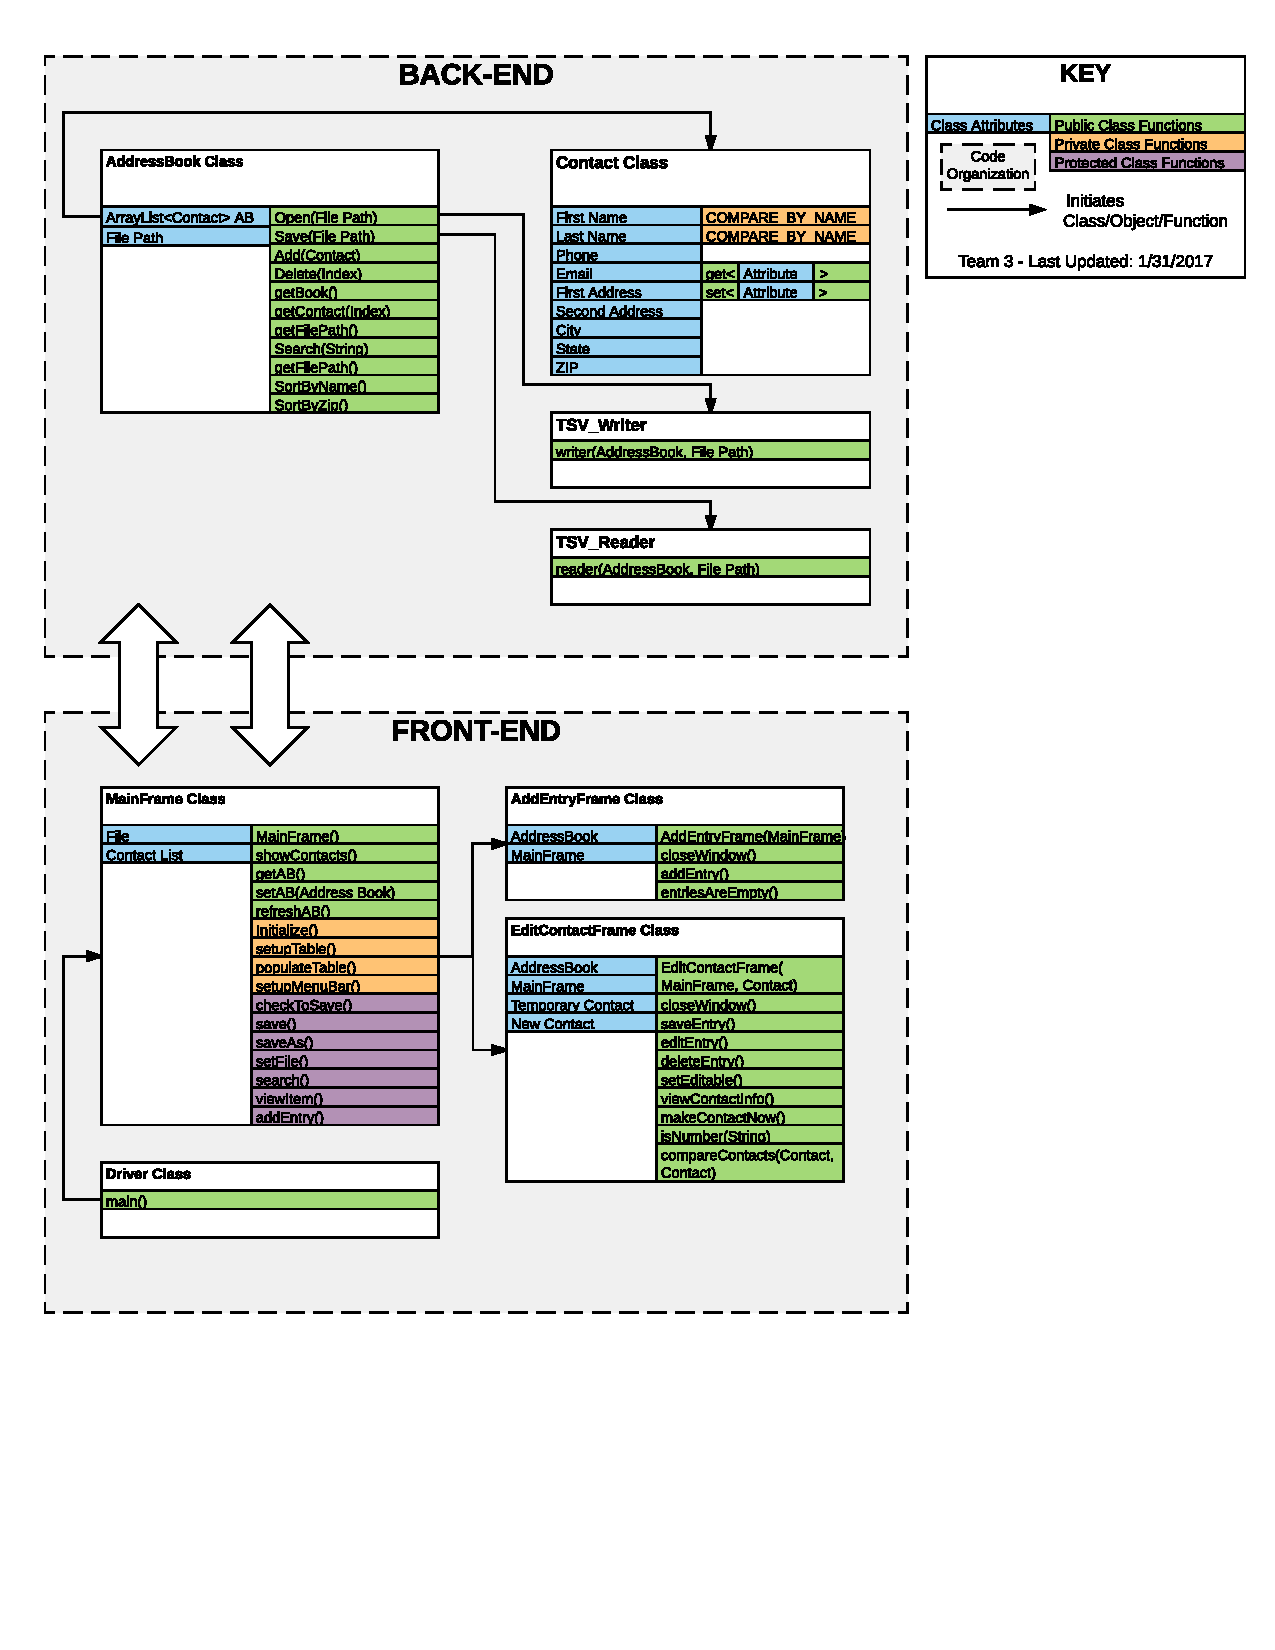
\includepdf[pages=-, offset=0 -50]{DesignDiagram.pdf}
\section{Introduction}
\subsection{Intended Audience}
The following document covers all functionality of the front and back end code and how they relate with the user's experience. This document is intended for programmers, team managers, and quality assurance on the developing team to ensure that the code is running to this specification.
\subsection{How to Use this Document}
This document is intended to help organize all modules, classes, and functions found in the Address Book code. It is meant to help all team members design their components to this specification, as well as having a straightforward method of analyzing interactions between different components. Reasonings for why design choices have been made are found at the end of the document.
\section{Summary}
The entirety of the program is based off of Java JDK 8, which is using a TSV file format to both load and export address book files. This document itself was created from the list of customer specifications which, with customer meetings, guided the creation of the Software Requirements Analysis, which was used to create the requirements needed to begin programming. This document will help create an Quality Assurance documents needed to test the quality of the resulting application. \\
This document will contain all programming interactions between modules, classes, and functions. This will be achieved by both diagrams and showing all function headers and descriptions of what they achieve and their interactions.
\section{User Interface Architecture}
\subsection{GUI Handbook}
\subsection{Expected Input}
The user is prompted to enter values for the following variables via text fields:
\begin{enumerate}[nolistsep]
	\setlength\itemsep{.1em}
	\item First name
	\item Last name
	\item Phone number
	\item Email
	\item Address: Street and 2nd Address
	\item City
	\item State
	\item ZIP code
\end{enumerate}
Other use inputs are included as buttons and from file menus, which are accessed by mouse clicks.
\begin{enumerate}[nolistsep]
	\setlength\itemsep{.1em}
	\item Close (Both program, and for adding a contact)
	\item Edit (Accessed by mouse clicking on a contact)
	\item Delete (Accessed within the edit contact menu)
	\item Search (Accessed by mouse clicking the search button next to the search bar)
	\item New (Accessed in file menu, creates and loads a new address book)
	\item Open (Accessed in file menu, opens an existing address book from a file directory)
	\item Save (Accessed in file menu, )
	\item Save As... (Accessed in file menu)
	\item Quit (Accessed in file menu, quits application completely.)
\end{enumerate}
\subsubsection{Output}
The user receives a list of contacts that they are able to view through, by scrolling a scroll bar on the side of the menu. They are able to access any visible contact by mouse clicks, and able to sort through this displayed list by sorting or searching. A user is allowed to edit or add a contact, which once changed can be elected to be saved and added to the current address book for future use. Upon loading any address book the current address book will be updated visually with the new address book.
\subsection{GUI Window}
\lstinputlisting[language=Java]{./exampleCode/AddressEntryFrame.java}
\lstinputlisting[language=Java]{./exampleCode/AddressEntryFrame2.java}

\subsubsection{Buttons}
\lstinputlisting[language=Java]{./exampleCode/deleteButton.java}
\lstinputlisting[language=Java]{./exampleCode/editButton.java}
\lstinputlisting[language=Java]{./exampleCode/newEntry.java}
\lstinputlisting[language=Java]{./exampleCode/addEntry.java}
\lstinputlisting[language=Java]{./exampleCode/closeWindow.java}
\subsection{Back-End Architecture}
\subsection{Contact Class}
The contact class is where all data regarding each entry in the address is kept. This class utilizes strings to hold all information about each entry. 
\subsubsection{Attributes of Contact Class}
\lstinputlisting[language=Java]{./exampleCode/contactClass.java}
\textit{This class holds the String data for first name, last name, phone number, email, address, 2nd address, city, state, and ZIP code.}
\subsubsection{Functions of Contact Class}
\textit{Functions: All Getters and Setters for Contact Class}\\
\textit{Precondition: \\Caller has a Contact Object if using a getter, or a String and a Contact object for input as a setter.}
\textit{Postcondition: All getters will return a String, all setters will return void, but set the inputted String for the corresponding contact.}
\lstinputlisting[language=Java]{./exampleCode/first.java}
\lstinputlisting[language=Java]{./exampleCode/last.java}
\lstinputlisting[language=Java]{./exampleCode/phone.java}
\lstinputlisting[language=Java]{./exampleCode/email.java}
\lstinputlisting[language=Java]{./exampleCode/address.java}
\lstinputlisting[language=Java]{./exampleCode/city.java}
\lstinputlisting[language=Java]{./exampleCode/state.java}
\lstinputlisting[language=Java]{./exampleCode/zip.java}

\subsubsection{AddressBook Class}
\textit{This class contains an arraylist of Contact objects and a few series of functions that allow different manipulations of these list of Contact objects. On constructing an Address Book, an ArrayList of Contacts is created and the following functions can be applied to this Address Book object:}
%\lstinputlisting[language=Java]{./exampleCode/createAddress.java}
\lstinputlisting[language=Java]{./exampleCode/save.java}
\textit{Functions: Save}\\
\textit{Precondition: String of intended file path for AddressBook object to be exported to.}\\
\textit{Postcondition: A boolean value, True if save was successful.}
\lstinputlisting[language=Java]{./exampleCode/add.java}
\textit{Functions: Add}\\
\textit{Precondition: A Contact Object}\\
\textit{Postcondition: Inputted Contact is saved into the applied Address Book.}
\lstinputlisting[language=Java]{./exampleCode/delete.java}
\textit{Functions: Delete}\\
\textit{Precondition: An Integer Index of the desired Contact to delete}\\
\textit{Postcondition: The Contact at the specific instance will be deleted from the Address Book.}
\lstinputlisting[language=Java]{./exampleCode/searchBy.java}
\textit{Functions: Search}\\
\textit{Precondition: An Address Book and an inputted String to search for.}\\
\textit{Postcondition: An ArrayList of Contacts is returned, which will contain all Contacts with any set of the inputted String found in any of the Contacts fields. This will be displayed on the Main GUI window.}
\subsubsection{Sorting}
\lstinputlisting[language=Java]{./exampleCode/sortByName.java}
\lstinputlisting[language=Java]{./exampleCode/sortByZip.java}
\lstinputlisting[language=Java]{./exampleCode/compareName.java}
\lstinputlisting[language=Java]{./exampleCode/compareZip.java}

\section{Module/Class Explanations}

\subsection{Driver}
\subsection{MainFrame}
\subsection{AddEntryFrame}
\subsection{EditContactFrame}

\subsection{AddressBook}
\subsection{Contact}
\subsection{TSV\_Reader}
\subsection{TSV\_Writer}

\section{Appendices}

\subsection{Definitions and Acronyms}
\subsubsection{Definitions}
\subsubsection{Acronyms and Abbreviations}

	\begin{tabular}{ | m{1cm} | m{10cm} | } 
		\hline
		GUI & Graphical User Interface \\
		\hline
		SDS & Software Design Specification \\
		\hline
		SRS & Software Requirement Specification  \\
		\hline
		TSV & Tab-Separated-Values \\
		\hline
	\end{tabular}












\end{document}

